\chapter{Method}\label{ch:method}

As described in MEC, an effective way to visualize the transitions between two
clustering results is by using a bipartite graph, where each node represents a
cluster at a specific time point, and edges represent overlaps between clusters
across the two time steps. In this representation, each transition can be
characterized by its origin cluster(s), destination cluster(s), and the
corresponding transition type.

\begin{figure}[H]
    \centering
    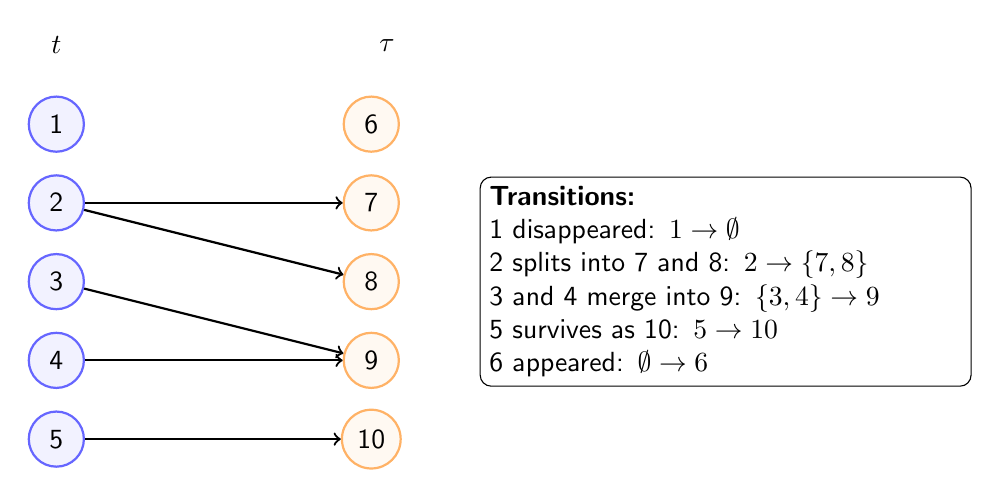
\begin{tikzpicture}[
            leftnode/.style={circle, draw=blue!60, fill=blue!5, thick, minimum size=7mm},
            rightnode/.style={circle, draw=orange!60, fill=orange!5, thick, minimum size=7mm},
            font=\sffamily,
            node distance=8mm and 30mm
        ]

        % Time labels
        \node[font=\bfseries] at (0,2) {$t$};
        \node[font=\bfseries] at (4.2,2) {$\tau$};

        % Left nodes (1 to 5)
        \node[leftnode] (n1) at (0,1) {1};
        \node[leftnode] (n2) at (0,0) {2};
        \node[leftnode] (n3) at (0,-1) {3};
        \node[leftnode] (n4) at (0,-2) {4};
        \node[leftnode] (n5) at (0,-3) {5};

        % Right nodes (6 to 10)
        \node[rightnode] (n6) at (4,1) {6};
        \node[rightnode] (n7) at (4,0) {7};
        \node[rightnode] (n8) at (4,-1) {8};
        \node[rightnode] (n9) at (4,-2) {9};
        \node[rightnode] (n10) at (4,-3) {10};

        % Edges
        \draw[->, thick] (n2) -- (n7);
        \draw[->, thick] (n2) -- (n8);
        \draw[->, thick] (n3) -- (n9);
        \draw[->, thick] (n4) -- (n9);
        \draw[->, thick] (n5) -- (n10);

        % Transitions legend centered vertically
        \node[align=left, anchor=center, text width=6cm, draw, rounded corners] (legend) at (8.5,-1) {
            \textbf{Transitions:} \\
            1 disappeared: $1 \rightarrow \emptyset$ \\
            2 splits into 7 and 8: $2 \rightarrow \{7, 8\}$ \\
            3 and 4 merge into 9: $\{3, 4\} \rightarrow 9$ \\
            5 survives as 10: $5 \rightarrow 10$ \\
            6 appeared: $\emptyset \rightarrow 6$
        };

    \end{tikzpicture}
    \caption{Example of transitions from clusters at time $t$ to clusters at time $\tau$.}
    \label{fig:cluster-transitions}
\end{figure}

To enable a precise and granular analysis, transitions such as splits and
merges are decomposed into atomic transitions that associate individual source
clusters with their respective destination clusters, or vice versa.

\begin{figure}[H]
    \centering
    \begin{minipage}{0.55\textwidth}
        \centering
        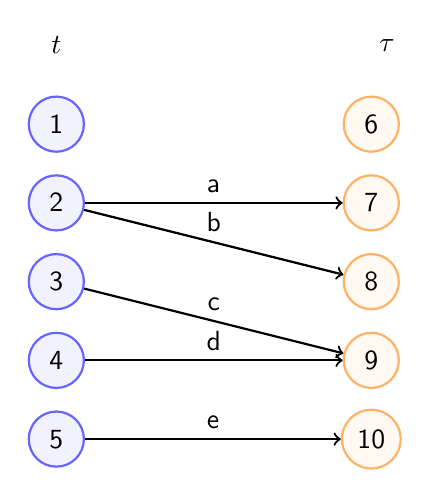
\begin{tikzpicture}[
                leftnode/.style={circle, draw=blue!60, fill=blue!5, thick, minimum size=7mm},
                rightnode/.style={circle, draw=orange!60, fill=orange!5, thick, minimum size=7mm},
                font=\sffamily,
                node distance=8mm and 30mm
            ]

            % Time labels
            \node[font=\bfseries] at (0,2) {$t$};
            \node[font=\bfseries] at (4.2,2) {$\tau$};

            % Left nodes (1 to 5)
            \node[leftnode] (n1) at (0,1) {1};
            \node[leftnode] (n2) at (0,0) {2};
            \node[leftnode] (n3) at (0,-1) {3};
            \node[leftnode] (n4) at (0,-2) {4};
            \node[leftnode] (n5) at (0,-3) {5};

            % Right nodes (6 to 10)
            \node[rightnode] (n6) at (4,1) {6};
            \node[rightnode] (n7) at (4,0) {7};
            \node[rightnode] (n8) at (4,-1) {8};
            \node[rightnode] (n9) at (4,-2) {9};
            \node[rightnode] (n10) at (4,-3) {10};

            % Edges
            \draw[->, thick] (n2) -- (n7) node[midway, above] {a};
            \draw[->, thick] (n2) -- (n8) node[midway, above] {b};
            \draw[->, thick] (n3) -- (n9) node[midway, above] {c};
            \draw[->, thick] (n4) -- (n9) node[midway, above] {d};
            \draw[->, thick] (n5) -- (n10) node[midway, above] {e};

        \end{tikzpicture}
    \end{minipage}
    \hfill
    \begin{minipage}{0.4\textwidth}
        \centering
        \begin{tabular}{|c|c|c|l|}
            \hline
            \textbf{Edge} & \textbf{From} & \textbf{To} & \textbf{Type} \\
            \hline
            -             & 1             & -           & Disappearance \\
            a             & 2             & 7           & Split         \\
            b             & 2             & 8           & Split         \\
            c             & 3             & 9           & Merge         \\
            d             & 4             & 9           & Merge         \\
            e             & 5             & 10          & Survival      \\
            -             & -             & 6           & Appearance    \\
            \hline
        \end{tabular}
    \end{minipage}
    \caption{Example of atomic cluster transitions between time $t$ and $\tau$.}
    \label{fig:atomic-cluster-transitions}
\end{figure}

Transitions between clusters can be characterized by analyzing the number of
edges connected to each node in the bipartite graph representation of
clustering results at times $ t $ and $ \tau $. Specifically:

\begin{itemize}
    \item For a cluster node at time $ t $:
          \begin{itemize}
              \item If it has no outgoing edges, the cluster is considered to have
                    \emph{disappeared}.
              \item If it has two or more outgoing edges, the cluster has undergone a \emph{split}.
          \end{itemize}
    \item For a cluster node at time $ \tau $:
          \begin{itemize}
              \item If it has no incoming edges, the cluster is considered to have \emph{appeared}.
              \item If it has two or more incoming edges, the cluster is the result of a
                    \emph{merge}.
          \end{itemize}
\end{itemize}

When a cluster node at either time $ t $ or time $ \tau $ is connected to
exactly one node at the other time point (i.e., has exactly one incident edge),
the type of transition cannot be determined solely based on that edge. In these
cases, additional context is required to disambiguate the type of transition.

\begin{itemize}
    \item From the perspective of time $ t $: If a cluster at time $ t $ has exactly one
          outgoing edge to a cluster at time $ \tau $, then:
          \begin{itemize}
              \item If the corresponding cluster at time $ \tau $ also has exactly one incoming
                    edge, the transition is a \emph{survival}.
              \item If the corresponding cluster at time $ \tau $ has more than one incoming edge,
                    the cluster at time $ t $ has merged with others into a single cluster.
          \end{itemize}

    \item From the perspective of time $ \tau $: If a cluster at time $ \tau $ has
          exactly one incoming edge from a cluster at time $ t $, then:
          \begin{itemize}
              \item If the originating cluster at time $ t $ also has only one outgoing edge, the
                    transition is a \emph{survival}.
              \item If the originating cluster at time $ t $ has more than one outgoing edge, it
                    has split into multiple clusters.
          \end{itemize}
\end{itemize}

When neither of the above conditions holds (i.e., a node at time $ t $ with one
edge connects to a node at time $ \tau $ that also participates in other
connections), the transition may involve both merging and splitting, which we
refer to as a \textbf{mergesplit}.

\begin{figure}[H]
    \centering
    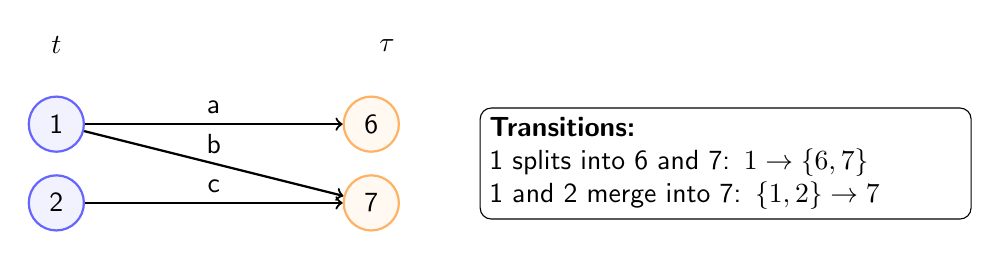
\begin{tikzpicture}[
            leftnode/.style={circle, draw=blue!60, fill=blue!5, thick, minimum size=7mm},
            rightnode/.style={circle, draw=orange!60, fill=orange!5, thick, minimum size=7mm},
            font=\sffamily,
            node distance=8mm and 30mm
        ]

        % Time labels
        \node[font=\bfseries] at (0,2) {$t$};
        \node[font=\bfseries] at (4.2,2) {$\tau$};

        % Left nodes
        \node[leftnode] (n1) at (0,1) {1};
        \node[leftnode] (n2) at (0,0) {2};

        % Right nodes
        \node[rightnode] (n6) at (4,1) {6};
        \node[rightnode] (n7) at (4,0) {7};

        % Edges
        \draw[->, thick] (n1) -- (n6) node[midway, above] {a};
        \draw[->, thick] (n1) -- (n7) node[midway, above] {b};
        \draw[->, thick] (n2) -- (n7) node[midway, above] {c};

        % Legend (left)
        \node[align=left, anchor=center, text width=6cm, draw, rounded corners] (legend) at (8.5,0.5) {
            \textbf{Transitions:} \\
            1 splits into 6 and 7: $1 \rightarrow \{6, 7\}$ \\
            1 and 2 merge into 7: $\{1, 2\} \rightarrow 7$
        };

    \end{tikzpicture}

    \vspace{1em}

    % Table below the diagram
    \begin{minipage}{0.8\textwidth}
        \centering
        \begin{tabular}{|c|c|c|l|}
            \hline
            \textbf{Edge} & \textbf{From} & \textbf{To} & \textbf{Transition Type} \\
            \hline
            a             & 1             & 6           & Split                    \\
            b             & 1             & 7           & Mergesplit               \\
            c             & 2             & 7           & Merge                    \\
            \hline
        \end{tabular}
    \end{minipage}
    \caption{Example of a mergesplit transition.}
    \label{fig:cluster-mergesplit}
\end{figure}

Up to this point, the discussed transitions have focused on comparisons between
clusters from two consecutive timestamps, capturing short-term structural
changes. However, to achieve more comprehensive tracking across longer time
horizons, it is beneficial to introduce three additional types of transitions
that account for recurring cluster behaviors: \textbf{reappearance},
\textbf{resplit}, and \textbf{remerge}.

\textbf{Reappearance} describes the event where a previously disappeared cluster
re-emerges at a later timestamp. To support the detection of this transition,
statistical information about disappeared clusters is stored. When a new cluster
appears in a future iteration, it is compared against the set of previously
disappeared clusters. If a significant overlap is found, the transition is
categorized as a reappearance rather than a new appearance.

\textbf{Remerge} refers to a scenario in which a cluster, originally formed by
the merging of multiple clusters, undergoes a subsequent split. In such cases,
information about the original merged components is preserved. If, at a later point,
the resulting clusters show sufficient overlap with the initially merged clusters,
the transition is identified as a remerge.

\textbf{Resplit} represents the inverse case, where clusters that were previously
the result of a split later merge again. The identities of the components resulting
from the original split are stored, and if these components recombine into a cluster
that significantly overlaps with the original one, the transition is recorded as a
resplit.

By incorporating these extended transition types, the tracking framework gains
the ability to identify not only immediate transformations but also long-term
structural recurrences, enabling a more nuanced understanding of cluster
evolution.

\begin{figure}[H]
    \centering
    \begin{tikzpicture}[node distance=1.5cm and 2cm, every node/.style={font=\small}]
        % Nodes
        \node (stream) [diamond, draw, minimum height=0.1cm, minimum width=5cm, above, inner sep=0pt] {Streaming Data};

        \node (online) [rectangle, draw, rounded corners, text centered, minimum height=1cm, below=2cm of stream] {\shortstack{Online\\(Microclustering)}};

        \node (offline) [rectangle, draw, rounded corners, text centered, minimum height=1cm, below=of online] {\shortstack{Offline\\(Macroclustering)}};

        \node (trigger) [rectangle, draw, rounded corners, text centered, minimum height=1cm, right=of online] {Triggering Strategy};

        \node (tracking) [rectangle, draw, rounded corners, text centered, minimum height=1cm, below=of offline] {Tracking};

        \node (history) [ellipse, draw, text centered, minimum height=1cm, left=of tracking] {History};

        \node (report) [diamond, draw, text centered, minimum height=1cm, minimum width=4cm, below=2cm of tracking] {Report};

        % Arrows
        \draw[thick,->,>=stealth] (stream) -- (online);
        \draw[thick,->,>=stealth] (online) -- (offline);
        \draw[thick,->,>=stealth] (trigger) |- (offline);
        \draw[thick,->,>=stealth] (offline) -- (tracking);
        \draw[thick,->,>=stealth] (offline) -| (history);
        \draw[thick,->,>=stealth] (history) -- (tracking);
        \draw[thick,->,>=stealth] (tracking) -- (report);

        % Box
        \node[draw, dashed, inner sep=10pt, fit=(online)(offline)(trigger), label=above right:Streaming Clustering] {};
        \node[draw, dashed, inner sep=45pt, fit=(online)(offline)(trigger)(history)(tracking), label=below left:Dynamic Clustering] {};

    \end{tikzpicture}
    \caption{Proposed architecture for the dynamic clustering framework.}
    \label{fig:architecture}
\end{figure}
